\documentclass[a4paper]{article}

\usepackage[english]{babel}
\usepackage[utf8]{inputenc}
\usepackage{amsmath}
\usepackage{graphicx}
\usepackage{caption}
\usepackage{subcaption}
\usepackage{listings}
\usepackage{algorithmic}
\usepackage[ruled]{algorithm2e} % For algorithms
\usepackage[colorinlistoftodos]{todonotes}
\usepackage[margin=1in]{geometry}
\usepackage{mathtools}
\DeclarePairedDelimiter\ceil{\lceil}{\rceil}
\DeclarePairedDelimiter\floor{\lfloor}{\rfloor}

\title{High Performance Computing and Big Data - OpenMP and MPI}

\author{Federico Tavella, Student number 11343605}

\date{\today}

\begin{document}
\maketitle

\section{Experimenting with OpenMP}

One of the main advantages of OpenMP is that it is not strictly necessary to change the source code to parallelise the program. In fact, we can improve the performances adding pragrams. Taking a look at the \texttt{multimult} function in Section~\ref{subsec:ausiliary}, we can see that the logic of the program is the same of the \texttt{multimult\_seq} function, which is the sequential version. We used the following macros to make the inner \texttt{for} loop parallel: \texttt{pragma omp parallel}, \texttt{private}, \texttt{shared} and \texttt{schedule}. By using \texttt{pragma omp parallel}, we are saying that different iterations of the loop can be executed in different threads. The \texttt{private} and \texttt{shared} macros define which are the variables shared among the different threads and which ones are not. In our case, the only private variable is \texttt{c}, which is used to temporarly store the value of the vector product between \texttt{a} and \texttt{b}. Finally, with the \texttt{schedule} macro we explicitly say in which order the different threads have to be executed; \texttt{static} means that the order is decided a priori of the execution, while the variable the second parameter for the \texttt{schedule} macro indicates the chunk size. Through different runs, we found out that the best results are obtained with $size_{chunk} = \dfrac{size_{array}}{n_{threads}}$.

One further improvement might be parallelising the external \texttt{for} loop, however this is not feasible without modifying the code because for each different iteration of this loop, the value of \texttt{a[i]} depends on the previous iterations. However, by switching the inner loop with the outermost one, we could make both of them run in parallel.

\subsection{Ausiliary functions}\label{subsec:ausiliary}

\begin{verbatim}
#include <stdio.h>
#include <unistd.h>
#include <stdlib.h>
#include <time.h>
#include <string.h>
#include "omp.h"

/*
  Function used to extract the number of seconds spent
*/

time_t extract_time_secs(struct timespec start, struct timespec stop){
  if(stop.tv_sec - start.tv_sec > 0 && stop.tv_nsec - start.tv_nsec < 0){
    return (stop.tv_sec - start.tv_sec - 1);
  }
  else{
    return (stop.tv_sec - start.tv_sec);
  }
}

/*
  Function used to extract the number of nanoseconds spent
*/

time_t extract_time_nsecs(struct timespec start, struct timespec stop){
  if(stop.tv_sec - start.tv_sec > 0 && stop.tv_nsec - start.tv_nsec < 0){
    return (1000000000 - (start.tv_nsec - stop.tv_nsec));
  }
  else{
    return (stop.tv_nsec - start.tv_nsec);
  }
}

/*
  Function used to start/stop the timer passed with clock_ref
*/

void get_time(struct timespec* clock_ref){
  if( clock_gettime(CLOCK_REALTIME, clock_ref) == -1 ) {
      perror( "clock gettime" );
      exit(-1);
  }
}

/*
  Function used to initialise the vectors
*/

void vectors_init(double* a, double* a_seq, double* b, int len){

  int dummy_value = 2;

  for(int i = 0; i < len; i++){
    a[i] = dummy_value;
    b[i] = dummy_value;
    a_seq[i] = a[i];
  }
}

/*
  Recursive function to calculate base^(expo)
*/

int powr(int base, int expo){
  if(expo == 0){
    return 1;
  }
  return base*powr(base, expo-1);
}

/*
  Sequential version of the multimult function
*/

void multimult_seq(double *a, double *b, int len, int steps){
  double c;
  for (int t=0; t < steps; t++){
    for (int i=0; i < len; i++){
        c = a [i] * b [i];
        a[i] = c * (double) t;
    }
  }
}

/*
  Parallel version of the multimult function
*/

void multimult(double *a, double *b, int len, int steps, int n_threads){
  double c;

  for (int t=0; t < steps; t++){
      #pragma omp parallel for private(c) shared(a,b,len,steps,t) \
      schedule(static, len/n_threads)
      for (int i=0; i < len; i++){
          c = a [i] * b [i];
          a[i] = c * (double) t;
      }
  }
}
\end{verbatim}

\subsection{Main function}

\begin{verbatim}
int main(){

  int step_iters = 10;    // number of iterations for the step variable
  int delta_steps = 10;   // delta at each iterations for the step variable
  int len_iters = 10;     // number of iterations for the length variable
  int delta_len = 50000;  // delta at each iterations for the length variable
  int thread_iters = 5;   // number of iterations for the threads variable

  // variable used to store the time of each iteration
  time_t results_seq_s[len_iters][step_iters];
  time_t results_seq_ns[len_iters][step_iters];
  time_t results_s[len_iters][step_iters][thread_iters];
  time_t results_ns[len_iters][step_iters][thread_iters];


    for(int k = 0; k < len_iters; k++){

      int len = delta_len*(k+1);
      double a[len], b[len], a_seq[len];

      for(int m = 0; m < step_iters; m++){

        int steps = delta_steps*(m+1);
        vectors_init(a,a_seq,b,len);
        // timers for the sequential/parallel programs
        struct timespec start_seq, stop_seq, start, stop;

        get_time(&start_seq);
        multimult_seq(a_seq,b,len,steps);
        get_time(&stop_seq);

        results_seq_s[k][m] = extract_time_secs(start_seq,stop_seq);
        results_seq_ns[k][m] = extract_time_nsecs(start_seq,stop_seq);

        for(int n = 0; n < thread_iters; n++){

          int n_threads = powr(2,n+1);
          omp_set_num_threads(n_threads);

          get_time(&start);
          multimult(a,b,len,steps,n_threads);
          get_time(&stop);

          results_s[k][m][n] = extract_time_secs(start,stop);
          results_ns[k][m][n] = extract_time_nsecs(start,stop);
        }
    }
  }

  /* storing the results into two different csv files */
  FILE *fp;     // file for the sequential results
  FILE *fp_par; // file for the parallel results

  fp=fopen("res_seq.csv", "w");
  if(fp == NULL)
      exit(-1);
  fprintf(fp, "length,steps,seconds,nanoseconds\n");

  fp_par=fopen("res.csv", "w");
  if(fp_par == NULL)
      exit(-1);
  fprintf(fp_par, "length,steps,threads,seconds,nanoseconds\n");

  for(int k = 0; k < len_iters; k++){
    for(int m=0; m < step_iters; m++){
      fprintf(fp,"%d,%d,%ld,%ld\n",delta_len*(k+1),delta_steps*(m+1),
              results_seq_s[k][m],results_seq_ns[k][m]);
      for(int n=0; n < thread_iters; n++){
        fprintf(fp_par,"%d,%d,%d,%ld,%ld\n",delta_len*(k+1),delta_steps*(m+1),
                powr(2,n+1),results_s[k][m][n],results_ns[k][m][n]);
      }
    }

  }

  fclose(fp)
  fclose(fp_par);

  return 0;
}
\end{verbatim}

\newpage

\subsection{Results}

%Specify characteristics of the processor
In this section, we describe the results obtained from different simulation runs on both laptop and Cartesius supercomputer. The computer on which the tests are executed is equipped with \texttt{Intel Core i7-3630QM CPU @ 2.40GHz x 8} processor, which means that it can run up to 8 threads simultaneously (4 physical processors and 8 virtual ones). In the following graphs, we use a logarithmic scale for the execution time in order to improve the readibility.

In Figure~\ref{fig:seq}, we can see how the number of elements in the array and the number of steps affect the execution time. There is a clear positive correlation between these two factor and the time required from the program to terminate. Moreover, we can see how the results on the local machine are more chaotic (i.e., with a less linear behaviour) than the ones obtained from Cartesius. We suppose this is due to interference of other processes during the simulation on the normal computer.

We can see how there is no significative difference between using the array length or the number of steps as abscissa. Consequently, from now on, we will always consider as x-axis the number of steps. In this way, we should get an indication of how much the parallelisation is improving the performance by looking at the distance between the different lines - i.e., how much the time is increasing with different vectors length.  

\begin{figure}[htbp]
\centering
\begin{subfigure}{.45\textwidth}
  \centering
  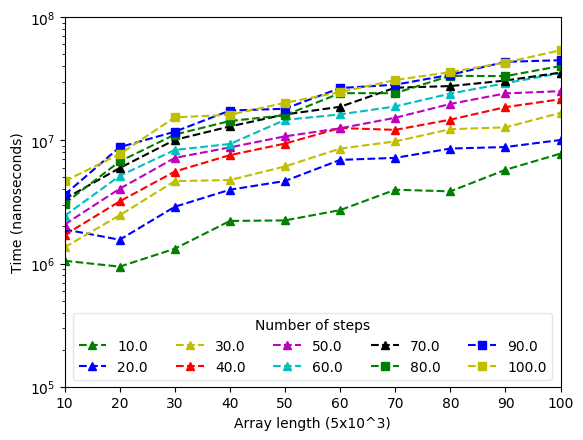
\includegraphics[width=\linewidth]{res/seq/array_length_res_seq.png}
  \caption{Run on local machine}
  \label{subfig:length_seq}
\end{subfigure}%
\begin{subfigure}{.45\textwidth}
  \centering
  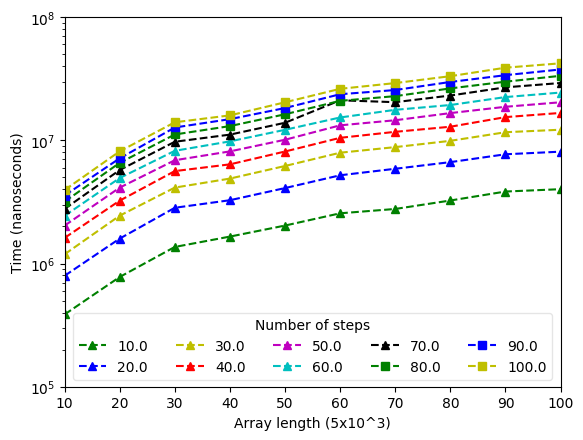
\includegraphics[width=\linewidth]{res/seq/array_length_res_seq_cartesius.png}
  \caption{Run on Cartesius}
  \label{subfig:length_seq_cart}
\end{subfigure}
\begin{subfigure}{.45\textwidth}
  \centering
  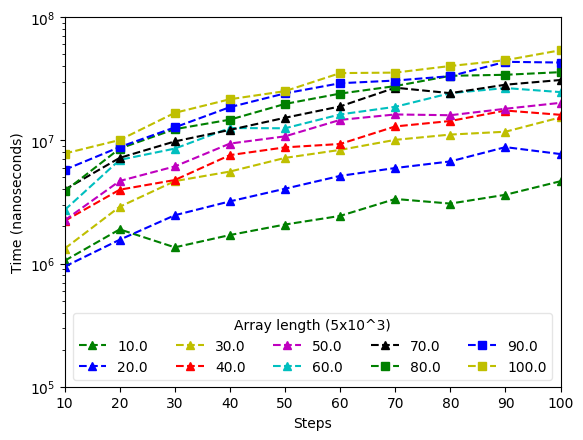
\includegraphics[width=\linewidth]{res/seq/array_steps_res_seq.png}
  \caption{Run on local machine}
  \label{subfig:steps_seq}
\end{subfigure}%
\begin{subfigure}{.45\textwidth}
  \centering
  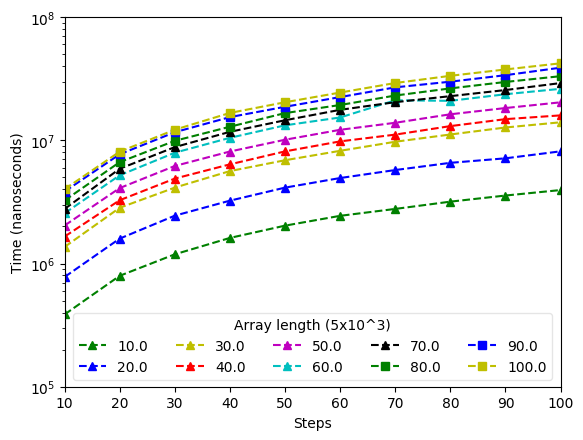
\includegraphics[width=\linewidth]{res/seq/array_steps_res_seq_cartesius.png}
  \caption{Run on Cartesius}
  \label{subfig:steps_seq_cart}
\end{subfigure}
\caption{Correlation between array length, number of steps and execution time - sequential version}
\label{fig:seq}
\end{figure}

Secondly, we want to verify that there is an improvement in the performance of the program when we increase the number of threads. However, this enhancement has an upper bound dictated by the number of cores of the machine. For example, we can see that on a machine with 8 cores, it is better to use 8 threads (Figure~\ref{subfig:steps_thread2_parall}) instead of 16 (Figure~\ref{subfig:steps_thread16_parall}).

In general, we can assert that the number of threads decreases the execution time of our program. We can see how in Figure~\ref{subfig:steps_thread2_parall_cart}, \ref{subfig:steps_thread4_parall_cart}, \ref{subfig:steps_thread8_parall_cart} and \ref{subfig:steps_thread16_parall_cart} the lines indicating the execution time are getting lower and closer, indicating respectively a reduction of the required time and the improvement provided from the parallelisation to bigger arrays. Moreover, as for the sequential version, even in this case the behaviour on the local machine is not as much linear as on the supercomputer.


\begin{figure}[htbp]
\centering
\begin{subfigure}{.42\textwidth}
  \centering
  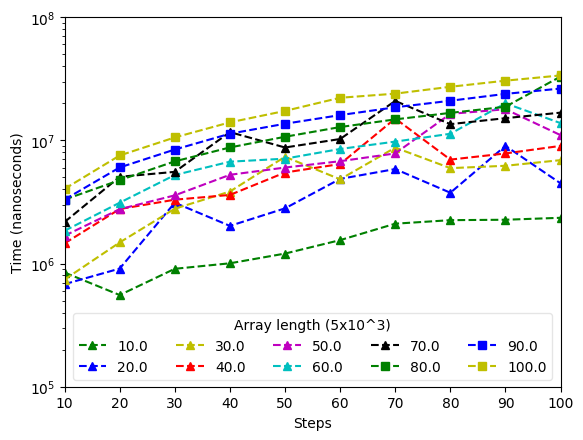
\includegraphics[width=\linewidth]{res/parallel/array_thread_2_steps_res.png}
  \caption{Local machine - 2 threads}
  \label{subfig:steps_thread2_parall}
\end{subfigure}%
\begin{subfigure}{.42\textwidth}
  \centering
  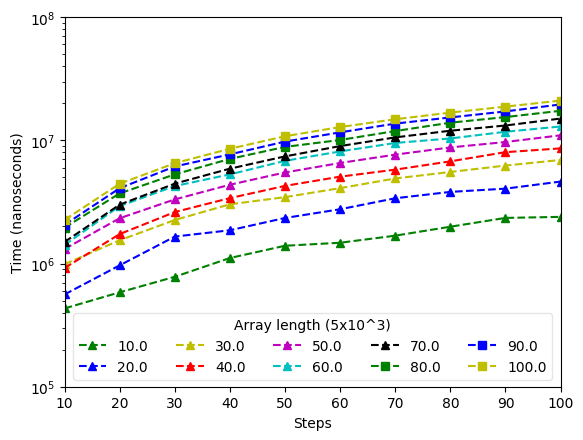
\includegraphics[width=\linewidth]{res/parallel/array_thread_2_steps_res_cartesius.png}
  \caption{Cartesius - 2 threads}
  \label{subfig:steps_thread2_parall_cart}
\end{subfigure}
\begin{subfigure}{.42\textwidth}
  \centering
  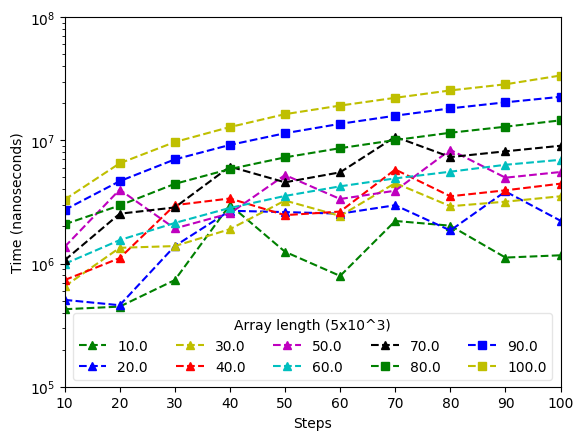
\includegraphics[width=\linewidth]{res/parallel/array_thread_4_steps_res.png}
  \caption{Local machine - 4 threads}
  \label{subfig:steps_thread4_parall}
\end{subfigure}%
\begin{subfigure}{.42\textwidth}
  \centering
  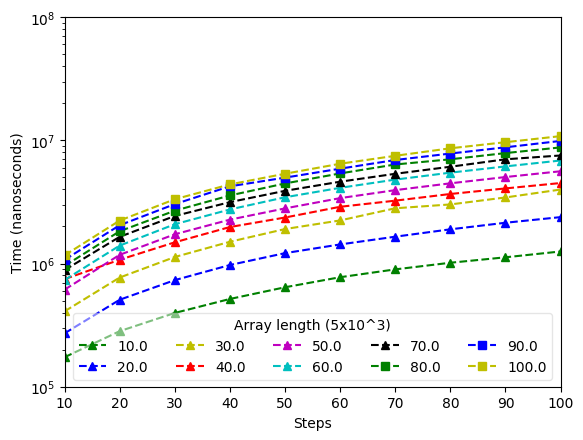
\includegraphics[width=\linewidth]{res/parallel/array_thread_4_steps_res_cartesius.png}
  \caption{Cartesius - 4 threads}
  \label{subfig:steps_thread4_parall_cart}
\end{subfigure}
\begin{subfigure}{.42\textwidth}
  \centering
  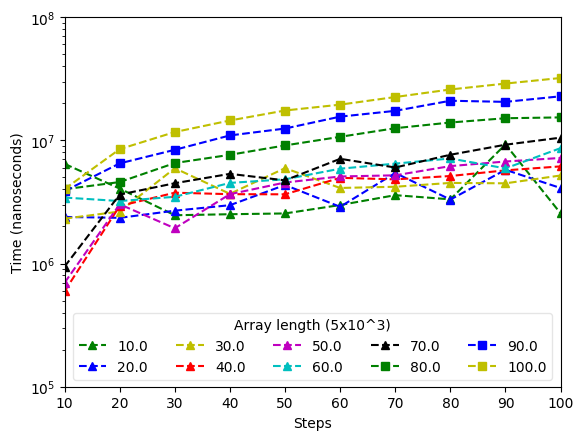
\includegraphics[width=\linewidth]{res/parallel/array_thread_8_steps_res.png}
  \caption{Local machine - 8 threads}
  \label{subfig:steps_thread8_parall}
\end{subfigure}%
\begin{subfigure}{.42\textwidth}
  \centering
  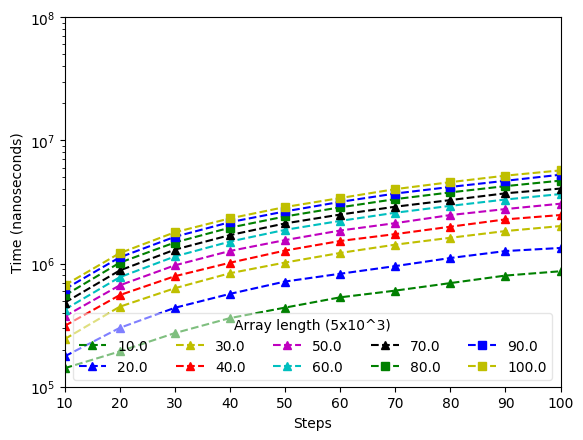
\includegraphics[width=\linewidth]{res/parallel/array_thread_8_steps_res_cartesius.png}
  \caption{Cartesius - 8 threads}
  \label{subfig:steps_thread8_parall_cart}
\end{subfigure}
\begin{subfigure}{.42\textwidth}
  \centering
  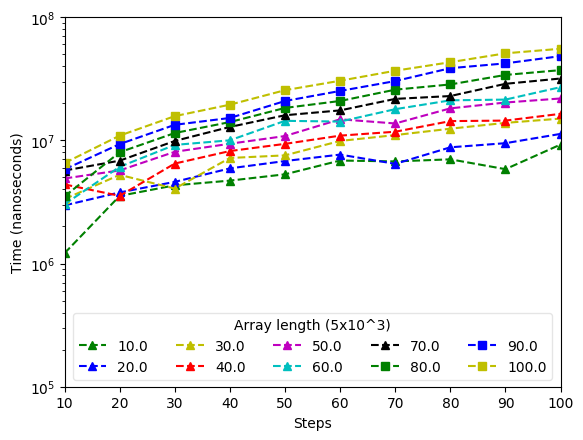
\includegraphics[width=\linewidth]{res/parallel/array_thread_16_steps_res.png}
  \caption{Local machine - 16 threads}
  \label{subfig:steps_thread16_parall}
\end{subfigure}%
\begin{subfigure}{.42\textwidth}
  \centering
  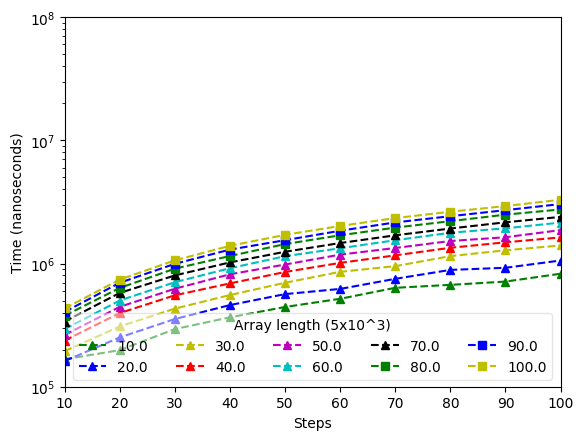
\includegraphics[width=\linewidth]{res/parallel/array_thread_16_steps_res_cartesius.png}
  \caption{Cartesius - 32 threads}
  \label{subfig:steps_thread16_parall_cart}
\end{subfigure}
\caption{Correlation between number of threads and execution time - parallel version}
\label{fig:steps_parall}
\end{figure}

Furthermore, in order to verify the upper bound previously defined, we executed one more simulation using 32 threads, knowing that the machine in Cartesius on which is executed has 16 cores. As a result, comparing Figure~\ref{subfig:steps_thread16_parall_cart} and Figure~\ref{fig:steps_thread32_parall_cart} it is evident that the execution time increases due to the overhead created by generating a number of threads greater than the number of cores.

\begin{figure}[htbp]
\centering
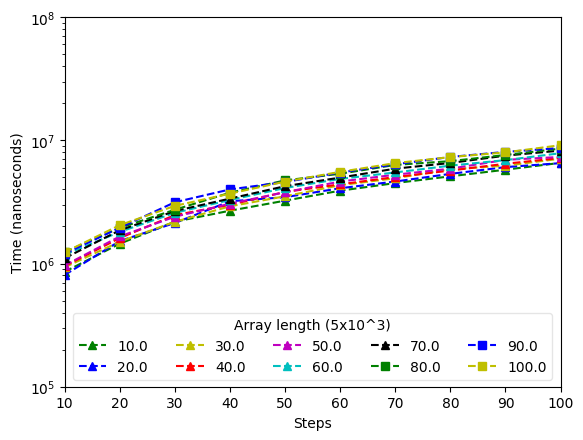
\includegraphics[width=0.7\textwidth]{res/parallel/array_thread_32_steps_res_cartesius.png}
\caption{Execution of the program with 32 threads on the Cartesius supercomputer}
\label{fig:steps_thread32_parall_cart}
\end{figure}
\newpage

\section{Collective communication}

In order to implement the collective communication, we can use the \texttt{MPI\_Send} and \texttt{MPI\_Recv} methods, First of all, we need to retrieve the communication \texttt{rank} and \texttt{size} (i.e., current process id and number of process respectively). To do so, we use the \texttt{MPI\_Comm\_rank} and \texttt{MPI\_Comm\_size} methods. Finally, if the current process is the root one, we broadcast the message to all the other process with the \texttt{MPI\_Send} method; otherwise, the current process is one of the receivers, so we start to listen awating for a message from the root process. The \texttt{tag} variable is used to filter messages from different process.

\begin{verbatim}
int MPI_Broadcast(  void *buffer,           /* INOUT : buffer address            */
                    int count,              /* IN    : buffer size               */
                    MPI_Datatype datatype,  /* IN    : datatype of entry address */
                    int root,               /* IN    : root process (sender)     */
                    MPI_Comm communicator)  /* IN    : communicator              */
{
  int rank, size, tag;
  MPI_Status status;
  MPI_Comm_rank(communicator, rank);
  MPI_Comm_size(communicator, size);

  //initialise tag variable

  if (rank == root) { // I am the root process
    for (int i = 0; i < size; i++) {
      if (i != rank) { //Avoid to send the message to myself
        MPI_Send(buffer, count, datatype, i, tag, communicator);
      }
    }
  }
  else { // I am a receiver process
    MPI_Recv(buffer, count, datatype, root, tag, communicator, &status);
    /* do something with the data */
  }
}

\end{verbatim}

\newpage

\section{Collective communication with topology adaptation}

Topology adaptation improved the performance of the broadcast communication, delegating the re-trasmission of the signal to other nodes. In the case of 1-dimensional ring topology, each node communicates with only two different nodes, one that has a greater MPI rank and one that has a smaller MPI rank than the node itself. Consequently, the root node send the message to its two neighboors, which propagates the message throught the ring without sending it back. In the end, there might be one or two nodes that are the last ones to receive the message, depending on the number of node of the network - i.e., if the number is even, there is one final node; otherwise, there are two.

If we assume $N$ is the number of nodes in the ring, there will be $N-1$ communication events (while without topology adaptation we would have $N$ events). However, since the broadcasting operation is distributed amoung the nodes, the time required to complete the broadcast is much smaller. If we consider as $k$ the time for a single \texttt{MPI\_Send} operation, without topology adaptation we need $kN$ time units to complete the broadcasting, but with this new feature the time is reduced to $k \cdot \floor*{\frac{N}{2}}$.

\begin{verbatim}
int MPI_Circular_Broadcast(  void *buffer,          /* INOUT : buffer address            */
                             int count,             /* IN    : buffer size               */
                             MPI_Datatype datatype, /* IN    : datatype of entry address */
                             int root,              /* IN    : root process (sender)     */
                             MPI_Comm communicator) /* IN    : communicator              */
{
  int rank, size, tag;
  MPI_Status status;
  MPI_Comm_rank(communicator, rank);
  MPI_Comm_size(communicator, size);

  //initialise tag variable

  int neighboor_lh, neighboor_rh;
  neighboor_rh = (rank + 1) % size;
  neighboor_lh = (rank - 1) % size;
  if (rank == root) { //Root process sends to neighboors
    MPI_Send(buffer, count, datatype, neighboor_lh, tag, communicator);
    MPI_Send(buffer, count, datatype, neighboor_rh, tag, communicator);
  }
  else if (rank < size/2){ // Circularly increasing MPI ranks
    MPI_Recv(buffer, count, datatype, neighboor_lh, tag, communicator, &status);
    // Send message to the neighboor that has bigger MPI rank
    MPI_Send(buffer, count, datatype, neighboor_rh, tag, communicator);
  }
  else if (rank > size/2){  // Circularly decreasing MPI ranks
    MPI_Recv(buffer, count, datatype, neighboor_rh, tag, communicator, &status);
    // Send message to the neighboor that has smaller MPI rank
    MPI_Send(buffer, count, datatype, neighboor_lh, tag, communicator);
  }
  else{ // Last nodes in the ring to reach

    /*
      By default, last node receive the message from the neighboor on its right
      in both cases size is even (one more node to reach) or odd (two nodes
      remaining)
    */

    MPI_Recv(buffer, count, datatype, neighboor_rh, tag, communicator, &status);
  }

  return 0;
}
\end{verbatim}

\end{document}